\documentclass{article}
\usepackage{geometry}
\geometry{a4paper, margin=1in}
\usepackage{enumitem}
\usepackage{graphicx}
\usepackage[hidelinks]{hyperref}
\usepackage{amsmath}
\usepackage{float}

\begin{document}

% Cover Page
\begin{titlepage}
	\centering
	\vspace*{1cm}

	
\includegraphics[width=0.5\textwidth]{assets/logo.png}\par\vspace{1cm} % Adjust the width as needed

	\Huge
	\textbf{Modeling Spatial Dependence: A Simulation-Based Comparison of Parametric and Semi-Parametric Approaches}

	\vspace{0.5cm}
	\LARGE
	Master in Statistics Mathematics

	\vspace{1.5cm}

	\textbf{Alejandro M. Ouslan}

	\vfill

	\Large
	Supervisors: \\
	Dr. Raul E. Macchiavelli \\
	Dra. Damaris Santana \\
	Dr. Julio C. Hernandez \\
	Dr. Roberto Rivera Santiago

	\vspace{0.8cm}

	\Large
	University of Puerto Rico, Mayagüez \\
	{\small \today}

\end{titlepage}

\newpage

\begin{abstract}
	This research aims to compare the performance of spatial regression models that rely on predefined weight matrices with that of semi-parametric regression models using spatial smoothers.
\end{abstract}

\section{Proposal Keywords}
Spatial simulation, Spatial Regressions, GAMs, Tensor Products

\section{Introduction}

Regression models are commonly used to simplify and represent complex real-world relationships. Since all models are approximations, additional components are often introduced to better capture underlying patterns. Spatial models are no exception and are not a novel concept. Through simulation, this research seeks to understand the limitations of various spatial models and identify contexts in which specific models are preferable.

We also aim to address key issues using Bayesian inference on one of the models. As a practical application, we will implement the models using data from the Quarterly Census of Employment and Wages (QCEW).

\section{Background and Motivation}

Spatial regression models are relatively simple yet expressive tools. The Spatial Durbin Model (SDM) can be expressed as:

\begin{equation}
	y = X \beta + \rho W X + \epsilon
\end{equation}

In this formulation, $X \beta$ represents the standard linear component, and $\rho W X$ incorporates spatial influence through a known weight matrix $W$. However, in real-world applications, $W$ is not truly known and must be inferred or chosen by the researcher. For example, $W$ can be represented in different forms, such as:

\begin{figure}[H]
	\centering
	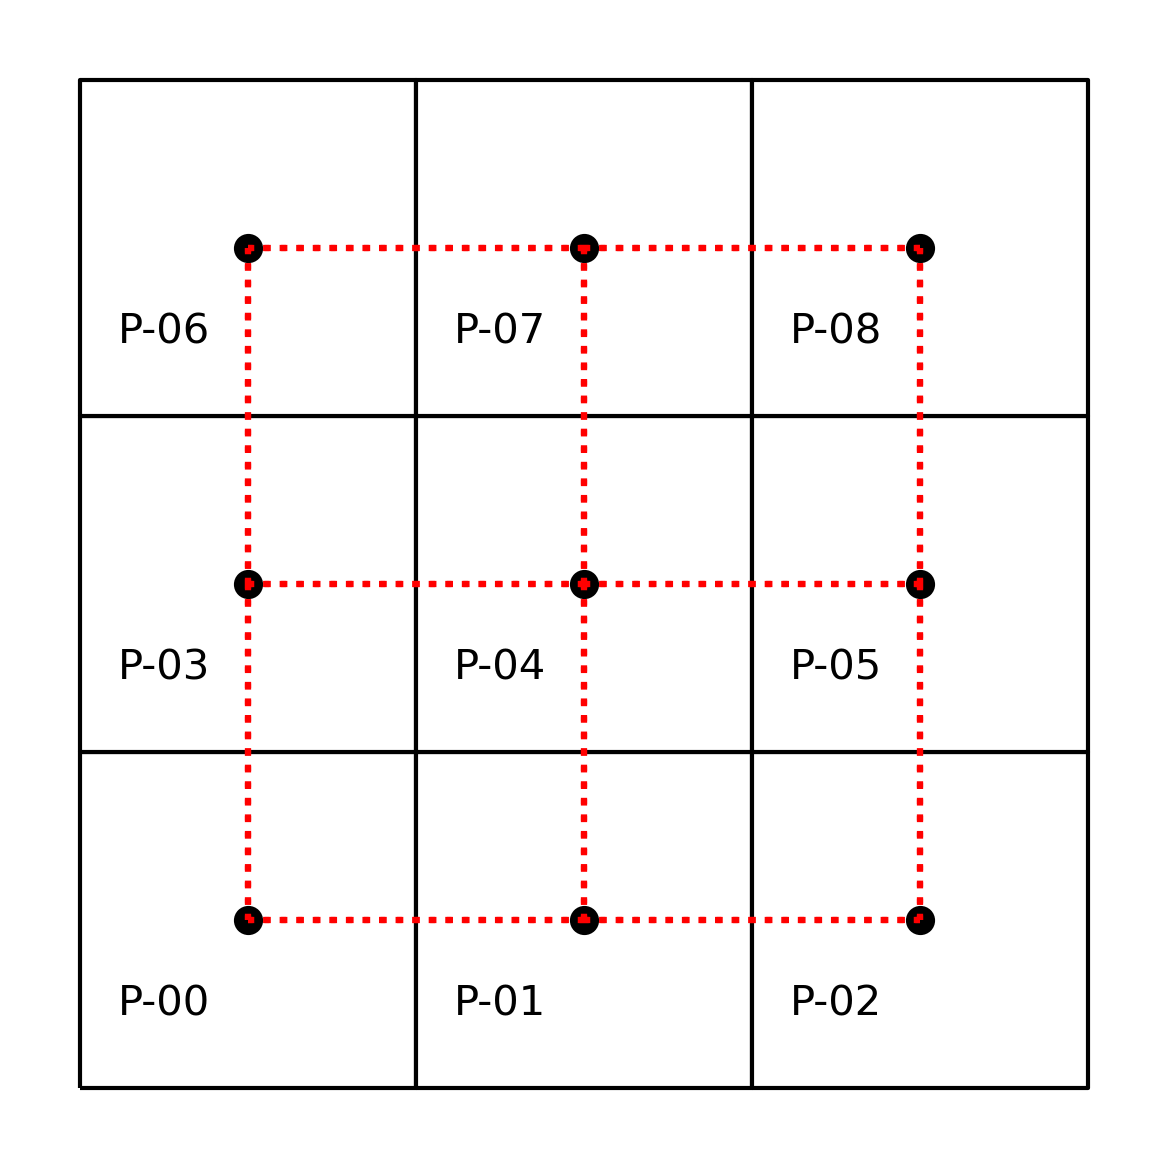
\includegraphics[width=0.4\textwidth]{assets/rook.png}
	\caption{Rook Contiguity Matrix}
\end{figure}

Mathematically, the rook model can be represented as:

\[
	\begin{bmatrix}
		0 & 1 & 0 & 1 & 0 & 0 & 0 & 0 & 0 \\
		1 & 0 & 1 & 0 & 1 & 0 & 0 & 0 & 0 \\
		0 & 1 & 0 & 0 & 0 & 1 & 0 & 0 & 0 \\
		1 & 0 & 0 & 0 & 1 & 0 & 1 & 0 & 0 \\
		0 & 1 & 0 & 1 & 0 & 1 & 0 & 1 & 0 \\
		0 & 0 & 1 & 0 & 1 & 0 & 0 & 0 & 1 \\
		0 & 0 & 0 & 1 & 0 & 0 & 0 & 1 & 0 \\
		0 & 0 & 0 & 0 & 1 & 0 & 1 & 0 & 1 \\
		0 & 0 & 0 & 0 & 0 & 1 & 0 & 1 & 0 \\
	\end{bmatrix}
\]

Another popular variant is the Queen’s contiguity model, which includes all bordering neighbors:

\begin{figure}[H]
	\centering
	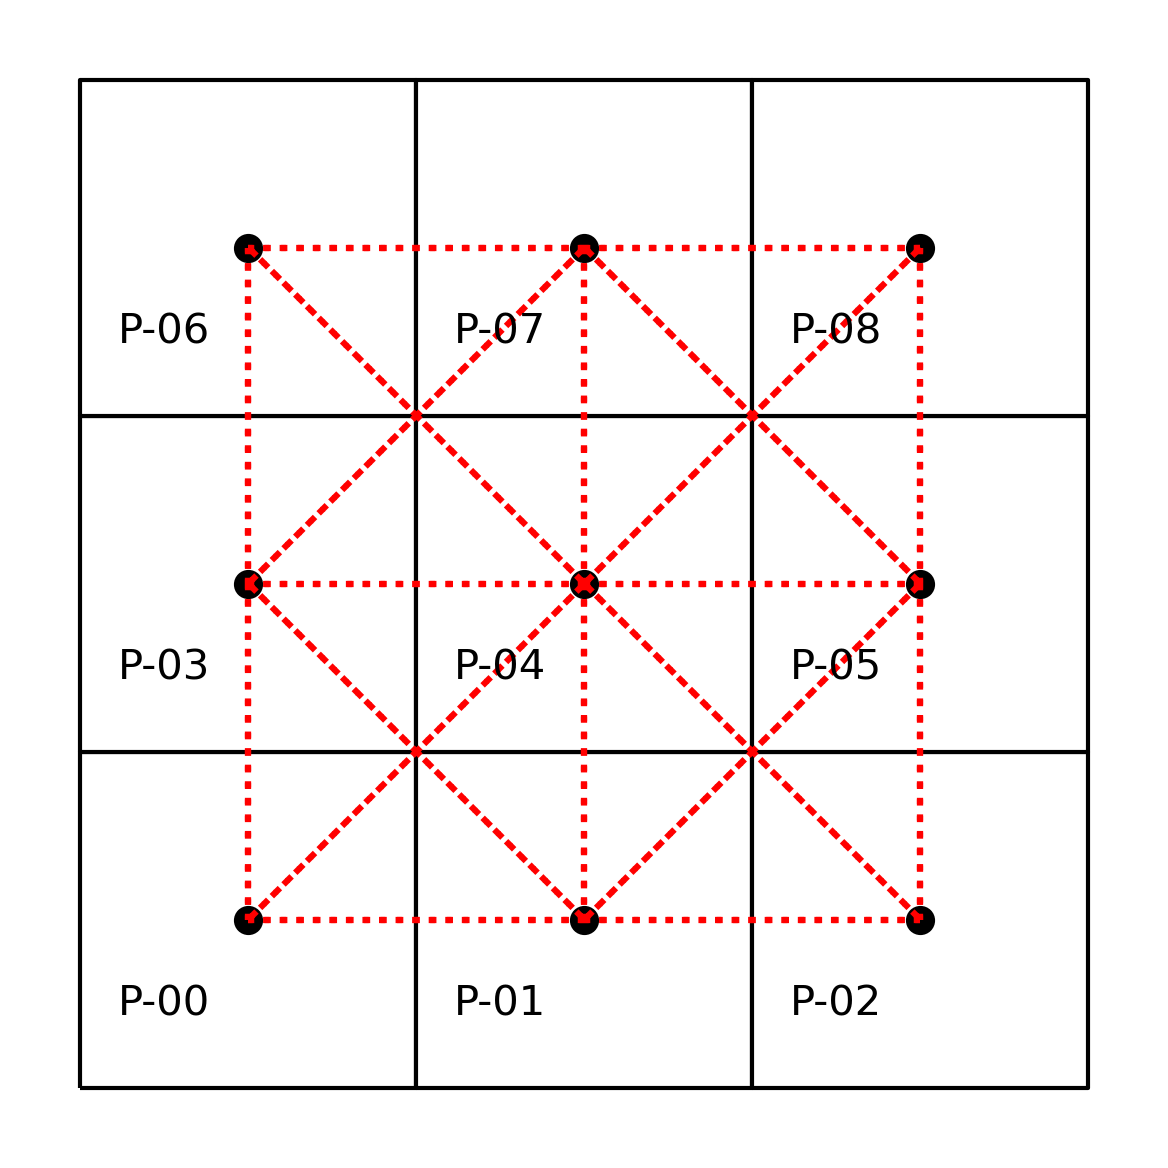
\includegraphics[width=0.4\textwidth]{assets/queens.png}
	\caption{Queen Contiguity Matrix}
\end{figure}

Its corresponding matrix:

\[
	\begin{bmatrix}
		0 & 1 & 0 & 1 & 1 & 0 & 0 & 0 & 0 \\
		1 & 0 & 1 & 1 & 1 & 1 & 0 & 0 & 0 \\
		0 & 1 & 0 & 0 & 1 & 1 & 0 & 0 & 0 \\
		1 & 1 & 0 & 0 & 1 & 0 & 1 & 1 & 0 \\
		1 & 1 & 1 & 1 & 0 & 1 & 1 & 1 & 1 \\
		0 & 1 & 1 & 0 & 1 & 0 & 0 & 1 & 1 \\
		0 & 0 & 0 & 1 & 1 & 0 & 0 & 1 & 0 \\
		0 & 0 & 0 & 1 & 1 & 1 & 1 & 0 & 1 \\
		0 & 0 & 0 & 0 & 1 & 1 & 0 & 1 & 0 \\
	\end{bmatrix}
\]

Another approach is the k-nearest neighbors (KNN) model, where influence decreases with distance:

\begin{figure}[H]
	\centering
	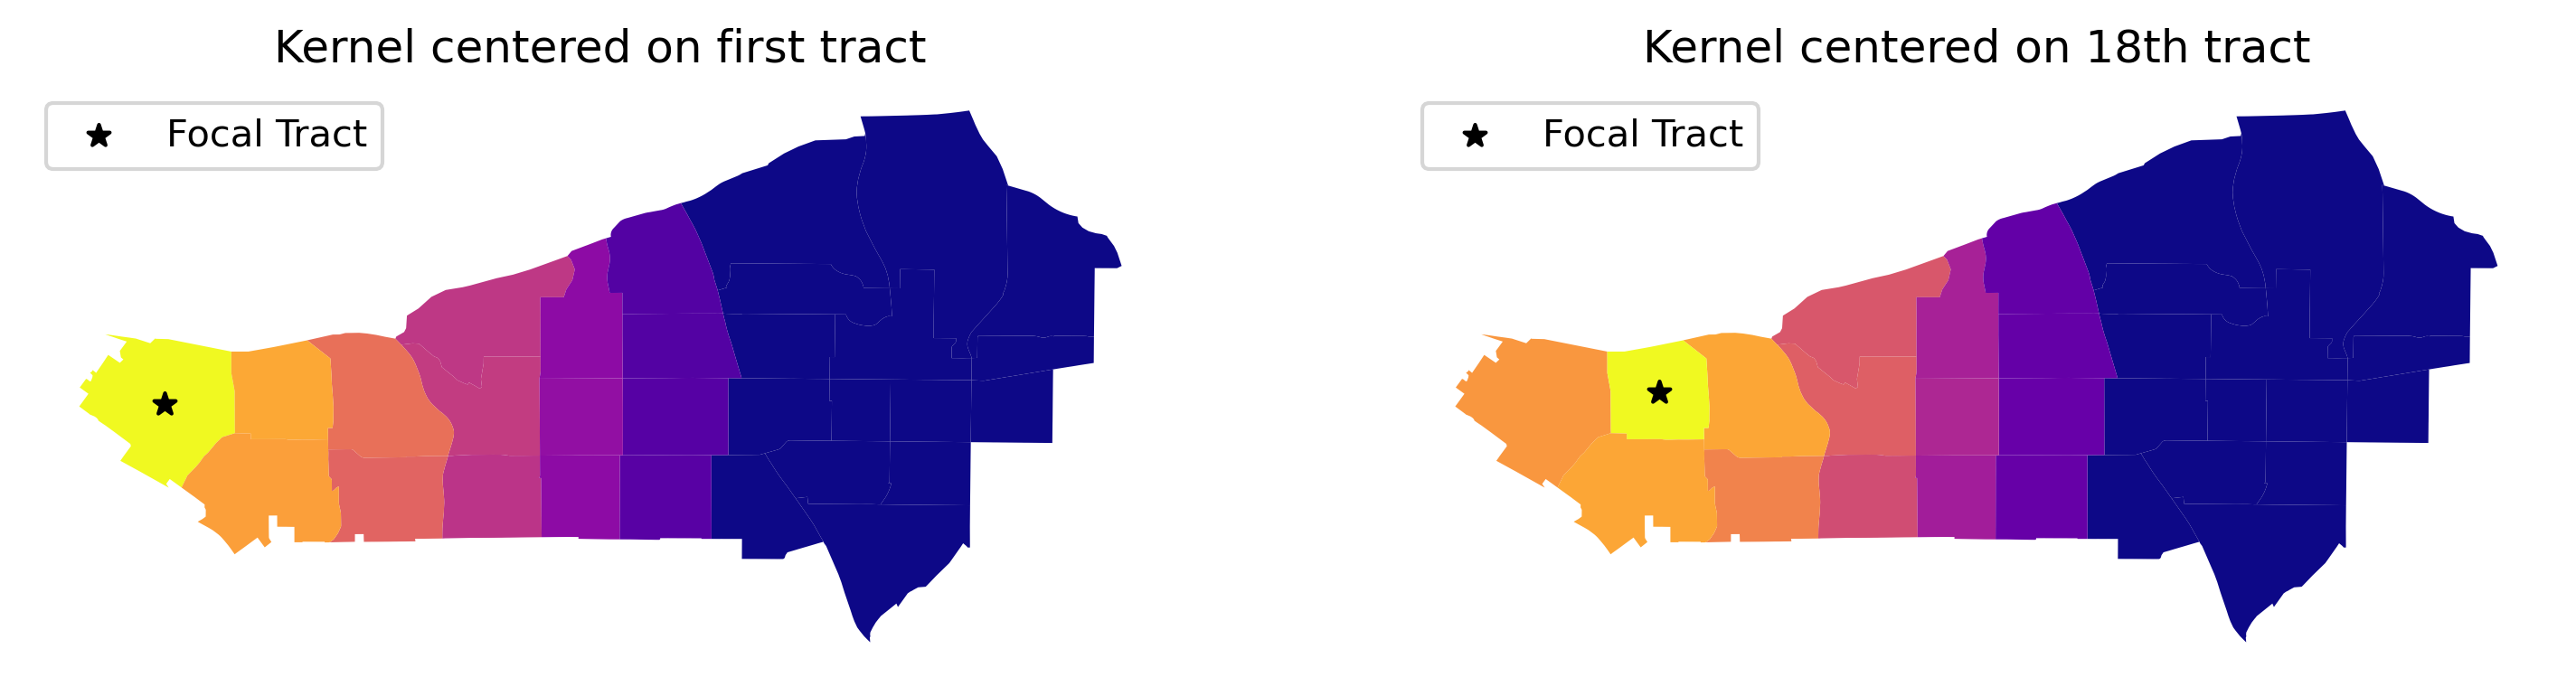
\includegraphics[width=0.64\textwidth]{assets/kmodel.png}
	\caption{K-Nearest Neighbors (KNN) Model}
\end{figure}

Clearly, there are numerous ways to define the $W$ matrix, and no universally accepted method exists for choosing the most appropriate one. In practice, $W$ is unknown and selecting it remains a major modeling challenge.

\section{Systematic Literature Review}

% [This section can be expanded with summaries of existing works and citations.]

\section{Aims and Objectives}

The primary objective of this research is to understand and compare the Spatial Durbin Model (SDM) and a semi-parametric model using tensor product smoothers. We will investigate under what circumstances each model performs better in terms of prediction accuracy and reliability. Furthermore, we aim to evaluate trade-offs such as ease of implementation, assumptions, computational cost, and interpretability.

We restate the SDM as:

\begin{equation}
	y = X \beta + \rho W X + \epsilon
\end{equation}

Where $W$ is predefined by the researcher, though in practice the actual spatial process remains unknown. Choosing an appropriate $W$ is often left to domain experts.

\section{Research Plan and Methodology}

We begin with the classical Ordinary Least Squares (OLS) regression:

\begin{equation}
	y_i = \alpha + \sum^p_{i=1} x_i \beta_i + \epsilon
	\label{eq:OLS}
\end{equation}

To account for spatial correlation, we introduce a spatial weight matrix $W$ into the regression:

\begin{equation}
	y = X \beta + \rho W X + \epsilon
	\label{eq:SDM}
\end{equation}

Which expands to:

\begin{equation}
	y_{it} = \alpha + \sum^p_{i=1} x_{it} \beta_i + \rho \sum^N_{j=1} w_{ij} x_{jt} + \epsilon
	\label{eq:SDM_exp}
\end{equation}

Alternatively, spatial terms may be incorporated into the dependent variable:

\begin{equation}
	y = \alpha + X \beta + \rho W Y + \epsilon
	\label{eq:SAR}
\end{equation}

Or into the error structure:

\begin{equation}
	\begin{split}
		y & = \alpha + X \beta + u  \\
		u & = \gamma W u + \epsilon
	\end{split}
	\label{eq:SEM}
\end{equation}

The semi-parametric model with a spatial smoother can be expressed as:

\begin{equation}
	y = \alpha + \sum^p_{i=1} x_{it} \beta_i + f(C_i) + \epsilon
	\label{eq:tensor}
\end{equation}

Where $C_i$ is the centroid of each observation and $f(C_i)$ is a spatial smoothing function.

We hypothesize that semi-parametric models may outperform spatial regression models, especially when the true $W$ matrix is unknown or misspecified.

\section{Prototype Design and Implementation}

We will simulate data using the following structure:

\begin{equation}
	y \sim \alpha + \sum^p_{i=1} x_{it} \beta_i + \rho \sum^N_{j=1} w_{ij} x_{jt} + \epsilon
\end{equation}

With $\epsilon \sim N(0,\sigma^2)$ and multiple forms of $W$ (rook, queen, KNN, etc.) used for robustness testing.

\section{Success and Impact}

SDM models are highly sensitive to the choice of $W$, for which no standardized selection method exists. Often, domain expertise is required. The semi-parametric model, however, does not depend on $W$, making it potentially more robust.

We will evaluate model performance using mean squared error (MSE) of predicted outcomes:

\begin{equation}
	\frac{\sum_{n=1}^N(y_n-\hat{y}_{nSDM})^2}{N}; \quad \frac{\sum_{n=1}^N(y-\hat{y}_{GAM})^2}{N}
	\label{eq:pref}
\end{equation}

And by comparing estimated vs. true coefficients:

\begin{equation}
	\frac{\sum_{n=1}^N(\beta-\hat{\beta}_{SDM})^2}{N}; \quad \frac{\sum_{n=1}^N(\beta-\hat{\beta}_{GAM})^2}{N}
	\label{eq:pref2}
\end{equation}

\newpage

\bibliographystyle{plain}
\bibliography{reference}

\end{document}
